\section{Additional Results and Interpretation}
\label{app:results}
\subsection{Structural contrasts and control scope}
\begin{table}[t]
\centering
\small
\begin{tabular}{llrr}
\toprule
Group & Estimator & $E_{\rm eq}$ & $E_{\rm rel,data}$ \\
\midrule
C7 & Joint & 0.0493 & 0.0135 \\
C7 & Ridge & 0.0483 & 0.0305 \\
C7 & Identity & 1.4458 & -- \\
C7 & Random orthogonal & 2.0297 & 1.8712 \\
\midrule
D4 & Joint & 0.0529 & 0.0097 \\
D4 & Ridge & 0.0520 & 0.0170 \\
D4 & Identity & 1.5300 & -- \\
D4 & Random orthogonal & 1.9978 & 1.9671 \\
\bottomrule
\end{tabular}
\caption{Held-out structural errors at $q=16$: descriptive means over six fixed models, four normalized depths, five splits, and six test templates per split. Lower is better. Random values average five controls; these controls are not independent model replications. Identity relation defects are intentionally not interpreted.}
\label{tab:structural-main}
\end{table}

\begin{table*}[t]
\centering
\small
\begin{tabular}{lrrl}
\toprule
Group & Composed & Direct & Composed minus direct [95\% interval] \\
\midrule
C7 & 0.0744 & 0.0511 & $0.0233\;[0.0040,\,0.0471]$ \\
D4 & 0.0566 & 0.0500 & $0.0065\;[0.0043,\,0.0094]$ \\
\bottomrule
\end{tabular}
\caption{Generator-only predictions of five never-independently-fitted elements on held-out templates ($q=16$). Direct Ridge fits each element separately and has lower error. The final column preserves the recorded 95\% bootstrap percentile interval; models form a fixed panel with overlapping partitions. These are resampling sensitivities, not calibrated population confidence statements (\cref{app:inference}).}
\label{tab:generator-transfer}
\end{table*}

\begin{figure}[t]
\centering
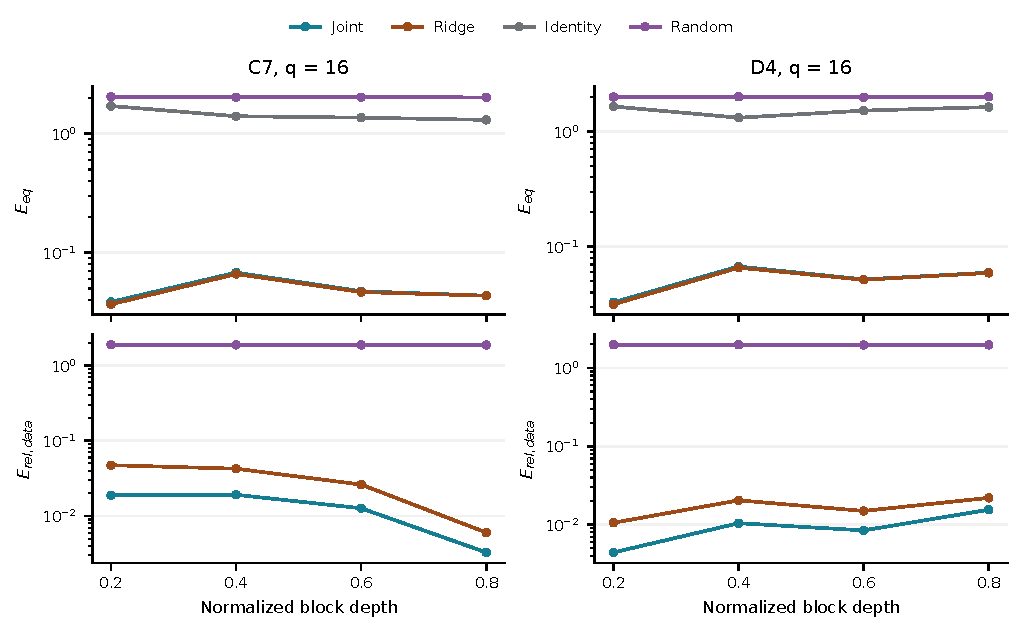
\includegraphics[width=.85\textwidth]{figures/structural_errors.pdf}
\caption{Historical direct prediction and relation consistency across the fixed six-model FULL panel at $q=16$. Joint fitting changes the prediction--consistency tradeoff; the diagnostics do not isolate semantic specificity.}
\label{fig:historical-structural}
\end{figure}
\begin{figure}[t]
\centering
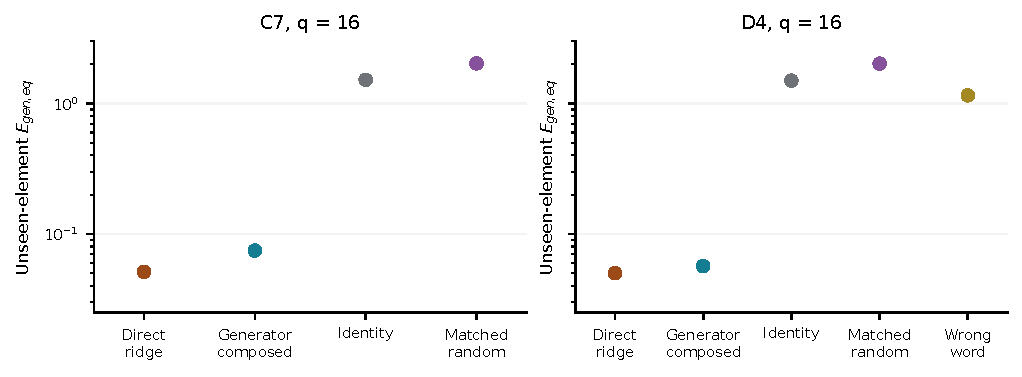
\includegraphics[width=.85\textwidth]{figures/generator_transfer.pdf}
\caption{Generator-only predictions evaluated against transformed held-out activations. Direct element-specific Ridge receives additional supervision. Identity, random generators and wrong words address distinct alternatives. These are the unchanged historical figure values.}
\label{fig:historical-generator}
\end{figure}
Joint relation defects decrease relative to Ridge by $-0.01699$ (recorded 95\% bootstrap interval $[-0.03405,-0.00318]$) for $C_7$ and $-0.00728$ ($[-0.01248,-0.00259]$) for $D_4$. For $D_4$, joint data relation components are $0.01717$ for $r^4$, $0.00876$ for $s^2$, and $0.00320$ for $srs=r^{-1}$. They are approximate relations on activations, not certification of exact ambient representations. In AFS-A, the correct-minus-wrong-word $D_4$ contrast is $-1.097329$ ($[-1.219881,-0.953809]$). All intervals retain the resampling-sensitivity scope of \cref{app:inference}.


The historical FULL joint-minus-random $\Eeq$ contrasts are $-1.9803$ ($[-2.0041,-1.9549]$) for $C_7$ and $-1.9449$ ($[-1.9562,-1.9325]$) for $D_4$. Joint-minus-identity values are $-1.3964$ ($[-1.5882,-1.1982]$) and $-1.4771$ ($[-1.6692,-1.2628]$). These large differences establish useful transformation prediction relative to untrained controls. The more demanding joint-minus-ridge prediction contrasts are slightly positive: $0.001046$ ($[0.000106,0.002285]$) and $0.000864$ ($[0.000149,0.001735]$). Joint-minus-ridge homomorphism differences are $-0.000884$ ($[-0.002083,-0.000018]$) and $-0.000891$ ($[-0.001652,-0.000232]$). These are effects under the historical resampling procedure; their small intervals do not resolve the identification alternatives in \cref{sec:boundaries}.


\begin{table}[h]
\centering
\small
\begin{tabular}{llccc}
\toprule
Group & Estimator & $\Ehom/\Ehomop$ & $\Erel/\Erelop$ & $\Ecomp/\Ecompop$ \\
\midrule
$C_7$ & Joint & 0.00842 / 0.05850 & 0.01348 / 0.09612 & 0.01145 / 0.07879 \\
$C_7$ & Ridge & 0.00930 / 0.06202 & 0.03047 / 0.20903 & 0.01266 / 0.08438 \\
$C_7$ & Random & 1.45937 / 1.03612 & 1.87118 / 1.45048 & 1.98636 / 1.41027 \\
$D_4$ & Joint & 0.00366 / 0.10143 & 0.00971 / 0.17124 & 0.00477 / 0.13149 \\
$D_4$ & Ridge & 0.00455 / 0.11897 & 0.01699 / 0.26283 & 0.00594 / 0.15530 \\
$D_4$ & Random & 1.52346 / 1.08021 & 1.96710 / 1.39203 & 1.98983 / 1.41088 \\
\bottomrule
\end{tabular}
\caption{Recorded primary FULL consistency diagnostics at dimension 16. Data/op pairs deliberately preserve distinct historical metrics: data defects are squared and op defects unsquared; C7 relation aggregands additionally differ. These paired columns should not be read as a comparison on one numerical scale. Homomorphism and composition differ only by excluding identity-containing pairs in the latter.}
\label{tab:full-diagnostics}
\end{table}

\begin{table*}[t]
\centering
\small
\begin{tabular}{lll}
\toprule
Control & Group/metric & Frozen summary \\
\midrule
AFS-B & C7, data homomorphism & 120/120 below reference 2.5th percentile \\
AFS-B & C7, operator homomorphism & 120/120 below reference 2.5th percentile \\
AFS-B & D4, data homomorphism & 120/120 below reference 2.5th percentile \\
AFS-B & D4, operator homomorphism & 120/120 below reference 2.5th percentile \\
AFS-C & C7, state relabel & $-0.577\;[-0.664,\,-0.488]$ \\
AFS-C & C7, target scramble & $-0.596\;[-0.686,\,-0.506]$ \\
AFS-C & D4, state relabel & $-0.765\;[-0.861,\,-0.662]$ \\
AFS-C & D4, target scramble & $-0.729\;[-0.824,\,-0.627]$ \\
\midrule
Global additive & Balanced complete orbit & $\widehat v_g=0$ by permutation cancellation \\
\bottomrule
\end{tabular}
\caption{Registration/correspondence controls and the scope of global additive falsification. AFS-C reports real-minus-scrambled test equivariance error after refitting on perturbed training pairs and scoring against unchanged true held-out targets; negative values favor the real correspondence. Brackets retain the historical bootstrap percentile intervals. AFS-B compares fixed operators with a restricted reference excluding automorphisms; observed and reference registrations are not established as exchangeable, so this is not calibrated semantic-null inference. The global displacement estimator averages complete state orbits and therefore reduces to identity independently of the activations.}
\label{tab:diagnostic-controls}
\end{table*}

AFS-B preserves the fitted matrix family while changing which algebraic element each matrix represents. AFS-C instead changes training correspondence while retaining the activation multiset, refits Ridge and scores it against the true held-out targets. In both groups and both scramble variants, the recorded mean test prediction and data-relation defects increase. The latter are consistency diagnostics on held-out activations, not additional semantic-target accuracy measurements. Prediction error and operator norms are not matched across conditions; moreover, the $C_7$ power-consistency and $D_4$ $srs$ terms normalize by condition-specific fitted outputs. The deterioration therefore does not isolate algebraic fidelity beyond the change in predictive fit. Neither AFS-B nor AFS-C demonstrates that a consistently registered alternative action of comparable learnability would fail.

\subsection{Rank-matched lexical comparison}
\begin{table*}[t]
\centering
\small
\begin{tabular}{lllrrr}
\toprule
Group & Model & Location & $E_{\rm eq}$ & $E_{\rm gen,eq}$ & $E_{\rm rel,data}$ \\
\midrule
C7 & Llama 1B & Embedding & $3.64\!\times\!10^{-6}$ & $5.87\!\times\!10^{-5}$ & $6.37\!\times\!10^{-5}$ \\
C7 & Llama 1B & Internal mean & 0.132327 & 0.198978 & 0.092076 \\
C7 & Qwen 1.5B & Embedding & $2.48\!\times\!10^{-6}$ & $4.25\!\times\!10^{-5}$ & $4.72\!\times\!10^{-5}$ \\
C7 & Qwen 1.5B & Internal mean & 0.171656 & 0.315743 & 0.187296 \\
D4 & Llama 1B & Embedding & $4.97\!\times\!10^{-7}$ & $2.97\!\times\!10^{-6}$ & $3.95\!\times\!10^{-6}$ \\
D4 & Llama 1B & Internal mean & 0.096634 & 0.133246 & 0.051652 \\
D4 & Qwen 1.5B & Embedding & $3.02\!\times\!10^{-7}$ & $1.80\!\times\!10^{-6}$ & $2.39\!\times\!10^{-6}$ \\
D4 & Qwen 1.5B & Internal mean & 0.055191 & 0.059383 & 0.027160 \\
\bottomrule
\end{tabular}
\caption{Rank-matched lexical control using independent Ridge, with generator-only composed predictions for $E_{\rm gen,eq}$. Both locations use C7 $q=6$ or D4 $q=3$; these are not the FULL $q=16$ estimates. Internal means average four fixed depths. Embedding errors are smaller in every tested model/group; all 150 archived internal-minus-embedding intervals are positive. Repeated templates at the embedding location reuse the same category vectors.}
\label{tab:lexical-control}
\end{table*}

\begin{figure}[h]
\centering
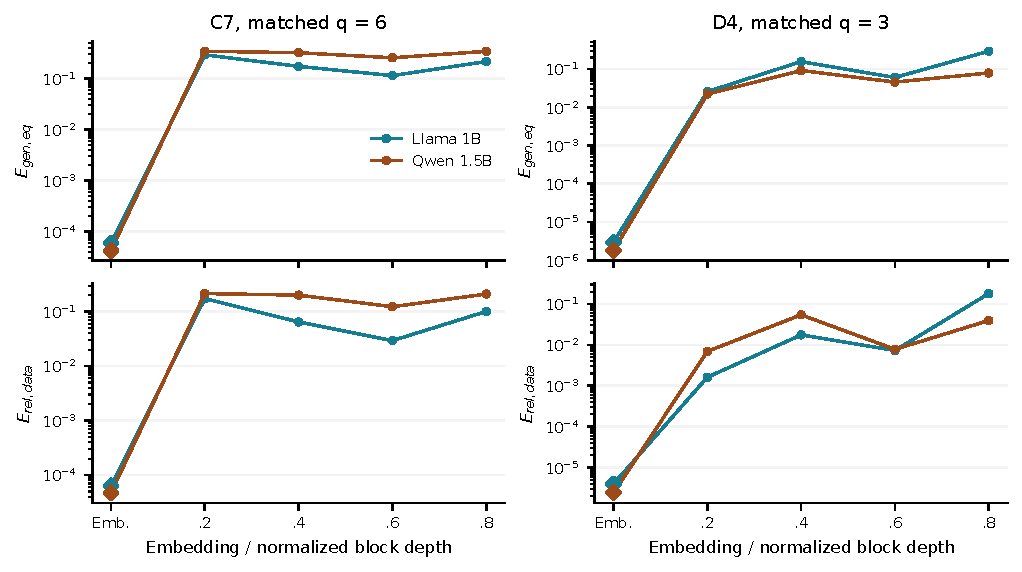
\includegraphics[width=0.76\textwidth]{figures/lexical_internal.pdf}
\caption{AFS-D independent fits at matched lexical ranks: $q=6$ for $C_7$, $q=3$ for $D_4$. This is a two-model comparison and not the dimension-16 primary FULL setting. Lexical near-exactness is compatible with finite-orbit realizability.}
\label{fig:lexical}
\end{figure}
Across the two models and two groups, the internal-minus-embedding contrasts are positive for both prediction and data relation error. This is evidence against internal strengthening in this recorded comparison. It is not evidence that embedding representations encode the uniquely correct semantic action; the full-rank lexical vectors permit every state permutation. Nor does it imply that arbitrary dimensions, models, reading positions, or contextual constructions behave identically.

\subsection{Global additive-field results}
The historical global-field direct errors are additive 1.487859, ridge 0.050149, and joint 0.051104. The additive-minus-ridge contrast is 1.437710 ($[1.400230,1.475673]$), and additive-minus-joint is 1.436755 ($[1.399237,1.474462]$). For repeated C7 generator prediction, the errors are 1.519200, 0.074443, and 0.070297. For the combined D4 paths $r\to s$, $s\to r$, and $s\to r\to s$, they are 1.266128, 0.049265, and 0.047450.

These are the completed experiment's observation-weighted means, not replacements for the FULL or AFS-A primary aggregates. The additive estimator cancels for every action because training covers complete, balanced state orbits. Repeated additive updates therefore cannot track even cyclic motion; for D4, they also cannot distinguish word orders because addition commutes. The reported descriptive order separation is 2.2133 for actual contextual targets, 2.2789 for ridge predictions, and 2.2526 for joint predictions, while the additive prediction has zero separation by construction. The first three are descriptive scores under the recorded normalization, not calibrated accuracies or independent confirmatory tests.

\subsection{Behavioral patching}
\label{app:behavior}
The evaluation prompt appends `` Report the transformed state:'' to a held-out structural prompt. The state remains visible, and the particular transformation is supplied through the selected activation intervention rather than by an explicit textual instruction naming $g$. Let $h$ be the mean state-span hidden vector from this evaluation prompt, $z=(h-\mu)C$, and $C$ the structural training-only PCA basis. The learned replacement is
\[
 h'=h-zC^\top+(zR_g)C^\top.
\]
The forward hook replaces every token position overlapping the state string with this replacement vector at the selected transformer block output, then recomputes the remaining network. If a state occupies multiple input tokens, all overlapping positions receive the same replacement derived from the mean; identity uses the original unpatched output. Thus an identity-matrix patch need not equal the unpatched baseline: overwriting distinct token vectors with their mean can itself change the network. The historical run does not contain a matched zero-delta, token-deviation-preserving sham. The one-token continuation counts below do not establish one-token source spans. These implementation details limit interpretation as a natural state substitution.

The source-conditioned additive comparator is trained from structural training prompts in the original hidden dimension:
\[
 v_{g,i}=\frac1{|\mathcal T_{\rm train}|}\sum_{t\in\mathcal T_{\rm train}}
 (h_{g(i),t}-h_{i,t}),\qquad h'=h+v_{g,i}.
\]
It uses known source-state identity and one vector per element/source pair, so it is more flexible than one source-shared linear operator. Its displacement also acts in the original hidden space, whereas the learned operator changes only the PCA component. The comparison therefore differs in source information, retained parameters and allowed edit subspace. It is an informative stronger comparator because it avoids orbit-averaging cancellation, but it is not a parameter- or subspace-matched test of steering optimality. In the recorded D4 relation rows the additive edit is indexed by the requested target element, so the true word, its direct reference and the wrong-word control receive the same endpoint-conditioned displacement; their equality for this comparator is built into the construction and does not test its composition order.

The target-token score uses the first token of the context-sensitive continuation `` \{target state\}''. Target logit change and target probability change subtract the unpatched prompt's values. The margin is target minus original-state first-token logit, and top-1 success requires the predicted vocabulary argmax to be that target token. The implementation records a full target-sequence log probability only for one-token continuations and would omit multi-token cases for that metric. All archived evaluated continuations contain one token. The scored top-1 outcome therefore concerns that continuation token; this experiment does not test general multi-token answer accuracy.

\begin{table*}[t]
\centering
\small
\begin{tabular}{llll}
\toprule
Group & Metric & Learned minus identity [95\% interval] & Learned minus additive [95\% interval] \\
\midrule
C7 & Target logit & $1.129\;[0.791,\,1.400]$ & $-0.105\;[-0.227,\,-0.014]$ \\
C7 & Top-1 (pp) & $1.743\;[-0.215,\,3.945]$ & $-0.261\;[-1.065,\,0.056]$ \\
D4 & Target logit & $2.406\;[1.932,\,2.833]$ & $-0.007\;[-0.030,\,0.012]$ \\
D4 & Top-1 (pp) & $9.019\;[3.186,\,15.339]$ & $-0.043\;[-0.503,\,0.434]$ \\
\midrule
\multicolumn{4}{l}{D4 correct-minus-wrong final-logit distance: $-0.0422\;[-0.0543,\,-0.0298]$.} \\
\bottomrule
\end{tabular}
\caption{Frozen behavioral contrasts from externally composed activation edits. Additive denotes the training-only source- and transformation-conditioned comparator, distinct from the global additive field. Positive logit/accuracy differences favor the learned edit; the D4 distance contrast is lower for the correct word. Top-1 measures the scored continuation token; all archived continuation counts are one. Recorded 95\% bootstrap percentile intervals preserve the original nested procedure; they describe fixed-panel resampling sensitivity, not calibrated population coverage (\cref{app:inference}).}
\label{tab:causal-main}
\end{table*}

\begin{figure}[h]
\centering
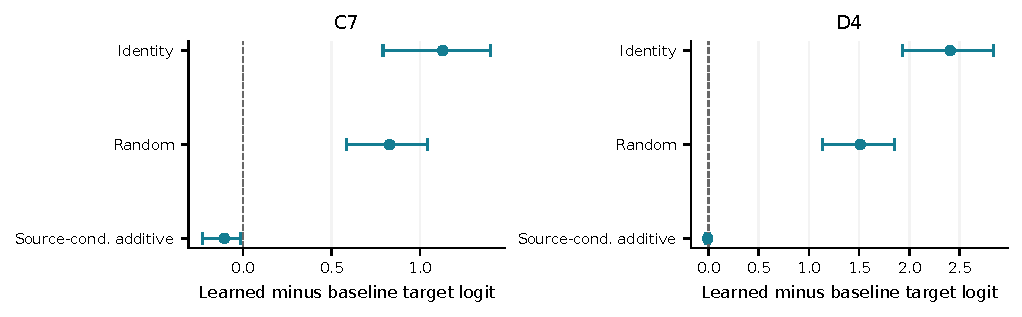
\includegraphics[width=0.76\textwidth]{figures/causal_additive.pdf}
\caption{Learned-minus-source-conditioned-additive target-logit effects. Negative differences favor the stronger additive comparator for that outcome. Directional behavioral effects do not demonstrate causal necessity of a recovered matrix family.}
\label{fig:causal}
\end{figure}
For C7, powers $r^1,\ldots,r^6$ are transformation interventions; $r^7$ is a separate cycle diagnostic. D4 tests $r,s,r^2,r^3$, identity-recovery words $r^4,s^2$, and the relation word $srs$ against a direct $r^{-1}$ intervention. The matched-length wrong word is $rsr$. For final next-token logit vectors $L$, the relation distance is
\[
 d(w,r^{-1})=\frac{\norm{L^{(w)}-L^{(r^{-1})}}_2}{\max(\norm{L^{(r^{-1})}}_2,\epsilon)}.
\]
The historical correct-minus-wrong distance difference is $-0.04220$ ($[-0.05426,-0.02981]$). Both words are evaluated relative to the same direct learned reference; this is an order-sensitive downstream consistency diagnostic, not comparison with a unique ground-truth causal mechanism. The C7 learned-minus-identity target-logit gain is 1.129 ($[0.791,1.400]$), and learned-minus-random is 0.828 ($[0.585,1.041]$). C7 top-1 evidence is weak. Learned-minus-additive target-logit intervals favor the additive baseline in C7 and include zero in D4. Together these observations support behavioral relevance with substantial causal ambiguity. Calendar interventions and competing group-operation mechanisms already demonstrate why an editable representation need not identify native computation \citep{engels2025notall,wu2025unified,feucht2026arithmetic}; the same caution applies to the externally composed edits here.

\FloatBarrier
\subsection{Cross-model compatibility}
Nine fixed pairs comprise all three within-Llama pairs, all three within-Qwen pairs, and size-matched cross-family pairs (1B/1.5B, 3B/3B, 8B/7B). For systems $R_A,R_B$, a row-coordinate map $T$ is assessed through
\[
 R_A(g)T\approx TR_B(g).
\]
The implementation writes $T=P^\top$, stacks the linear constraints $PR_A(g)^\top-R_B(g)^\top P$, takes the smallest right-singular-vector solution, and normalizes $\norm{P}_F=1$. It does not require $P$ to be invertible, well-conditioned, orthogonal, or high effective rank. The normalized score is
\[
 \frac{\mathbb{E}_g\norm{PR_A(g)^\top-R_B(g)^\top P}_F^2}
 {\mathbb{E}_g\norm{R_B(g)^\top P}_F^2+10^{-12}}.
\]
Comparators include an orthogonal Procrustes map estimated from registered activation correspondence, random orthogonal maps, and shuffled group labels. The Procrustes map is fitted on the reported test-template activation pairs and optimizes activation reconstruction, while the intertwiner optimizes commutation using the same group elements later scored. This is a descriptive comparison of two fitting criteria, not predictive transport to unseen paired activations or held-out elements. A low-rank common subspace may suffice. The shuffled-label control keeps the map fitted under true labels rather than refitting after shuffling; it tests sensitivity of that map to registration, not the best achievable fit under each alternative. Shuffled-label controls can also be near-degenerate.

Unlike implementation-family comparisons based on causal abstractions and Congruity \citep{sun2026tracking}, this experiment neither samples behavior-preserving implementations nor estimates their abstraction-dependent distance. The recorded fitted-minus-Procrustes residual differences range approximately from $-0.065$ to $-0.168$ over the registered strata, with historical intervals below zero. This establishes existence of lower-residual fitted commutation maps than the chosen geometry alignment on these elements, not cross-model representation equivalence. The recorded Spearman association with conventional linear CKA is $-0.014$ with interval $[-0.300,0.287]$, leaving that relationship unresolved.

\subsection{Completed controls and remaining identification scope}
The characterization supplies state-centroid, residual and input-only field comparisons under its own sampling and normalization contract. The returned extension additionally completes full-data compact nonlinear predictors, coherent alternative registration, direct context-difference fits and peer adaptations (\cref{app:reproduction}). Their descriptive results are now part of the evidence; they do not retroactively repair a historical comparison's information or intervention mismatch.

The remaining gaps concern stronger claims than the fixed-panel predictive account retained here: algebraic evidence beyond prediction would require a direct-error- and operator-norm-matched comparison; cross-vocabulary generalization would require genuinely new lexical realizations and independently authored context families; native causal use would require competent-task counterfactual evidence. Native confirmation remains blocked despite completed secondary adaptations. None of those stronger claims is inferred from the present comparisons. Future method selection on the inspected holdout would be exploratory and would need fresh evaluation before confirmation. A same-order wrong-group comparison also requires a feasible matched action: no four-state permutation has order eight, so $C_8$ cannot act faithfully on the four corners. An impossible alternative is not an error-matched semantic reference.
